\section{Results and Discussion}\label{sec:result}

\begin{figure*}
    \centering
    \begin{subfigure}[b]{0.495\textwidth}
    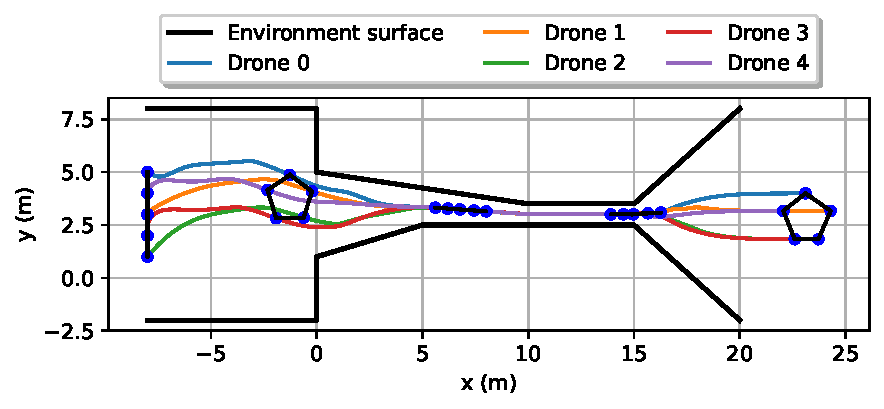
\includegraphics[width=\textwidth]{paper3/images/path_scen1.pdf}
    \caption{Scenario 1 - Motion paths}
    \end{subfigure}
    \begin{subfigure}[b]{0.495\textwidth}
    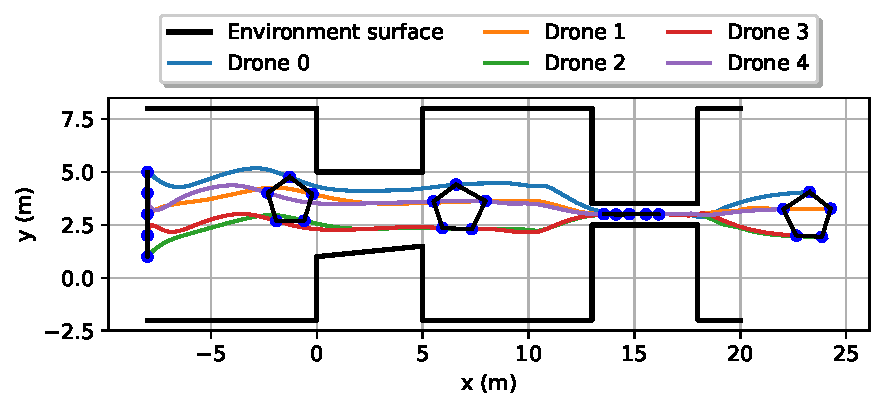
\includegraphics[width=\textwidth]{paper3/images/path_scen2.pdf}
    \caption{Scenario 2 - Motion paths}
    \end{subfigure}
    \begin{subfigure}[b]{0.495\textwidth}
    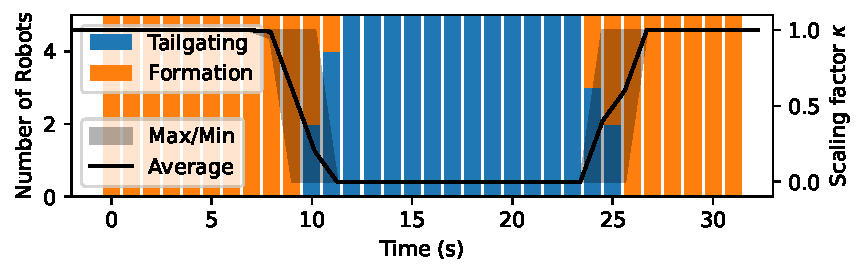
\includegraphics[width=\textwidth]{paper3/images/correlation_scen1.pdf}
    \caption{Scenario 1 - Correlation between the number of  robots (bar chart) in each mode and the scale factor (black line) over time}
    \label{fig:cor1}
    \end{subfigure}
    \begin{subfigure}[b]{0.495\textwidth}
    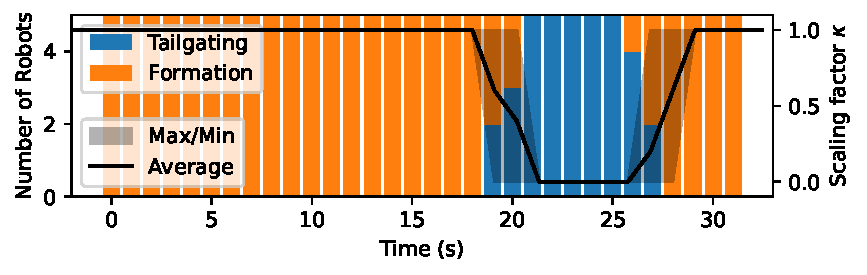
\includegraphics[width=\textwidth]{paper3/images/correlation_scen2.pdf}
    \caption{Scenario 2 - Correlation between the number of  robots (bar chart) in each mode and the scale factor (black line) over time}
    \label{fig:cor2}
    \end{subfigure}
    \caption{Trajectories and formation shapes of the robots controlled by the PRC in two evaluating scenarios.}
    \label{fig:path}
\end{figure*}

A number of simulations, comparisons, and software-in-the-loop tests have been conducted to evaluate the performance of the PRC with details as follows.

\subsection{Evaluation Setup}
The swarm includes five identical robots, each with a radius of $r=0.2$~m, a maximum speed of $\left\Vert \mathbf{v}_\text{max}\right\Vert=1.5$~m/s, and a maximum control input $\left\Vert \mathbf{u}_\text{max}\right\Vert=2.0$~m/s$^2$. The robot is equipped with a range sensor having the sensing range of $r_s=3$~m. The desired formation shape is set to a pentagon, the reference velocity is $v_\text{ref}=1$~m/s, and the desired direction is $\mathbf{u}_\text{ref}=[1,0,0]^T$. The environments include two structures, both having narrow passages, as depicted in Figure~\ref{fig:path}.

The metrics used for evaluation include the success rate, mean \textit{order} $\Phi$, mean speed (m/s), mean formation error $\varepsilon$ (m), and acceleration cost $\Gamma$ (m$^2$/s$^4$) \cite{Zhang2021}. The \textit{order} metric~\cite{Vicsek1995} measures the heading consensus of the robots and is computed as:
\begin{equation}
    \Phi=\dfrac{1}{N}\left\Vert\sum_{i=1}^N{\dfrac{\mathbf{v}_i}{\left\Vert \mathbf{v}_i\right\Vert}}\right\Vert
\end{equation}
Its value ranges from 0 to 1, with 1 indicating the robots have the same direction. The \textit{formation error} measures the deviation between the desired and actual positions of the robots and is calculated as~\cite{6798711}:
\begin{equation}
    \varepsilon_i = \left\Vert \mathbf{p}_i-\mathbf{p}^*_i\right\Vert
\end{equation} 
The acceleration cost indicates the control effort and is given by:
\begin{equation}
    \Gamma = \dfrac{1}{n}\sum_{i=1}^N{\left\Vert \mathbf{u_i}(k)\right\Vert^2}
\end{equation} 

The comparing methods include the behavior-based reconfiguration control (BRC) \cite{Vsrhelyi2018} and the predictive formation control (PFC)~\cite{9562281}. In evaluation, each method is run 10 times for each scenario.   

\subsection{Results}
\label{subsec:results}

\begin{figure*}
    \centering
    \begin{subfigure}[b]{0.495\textwidth}
    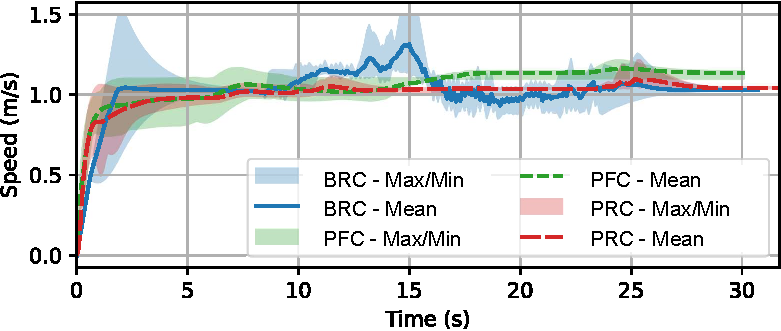
\includegraphics[width=\textwidth]{paper3/images/velocity_scen1.pdf}
    \caption{Scenario 1 - Speed}
    \label{fig:speed1}
    \end{subfigure}
    \begin{subfigure}[b]{0.495\textwidth}
    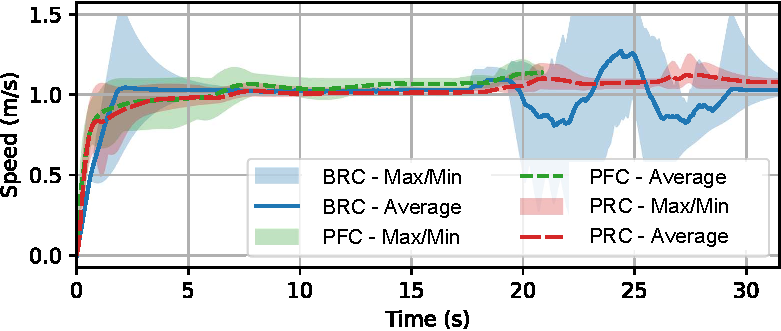
\includegraphics[width=\textwidth]{paper3/images/velocity_scen2.pdf}
    \caption{Scenario 2 - Speed}
    \label{fig:speed2}
    \end{subfigure}
    \begin{subfigure}[b]{0.495\textwidth}
    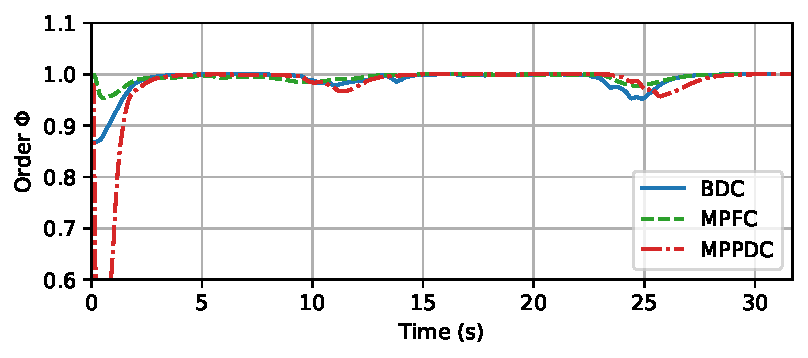
\includegraphics[width=\textwidth]{paper3/images/order_scen1.pdf}
    \caption{Scenario 1 - \textit{Order} $\Phi$}
    \label{fig:order1}
    \end{subfigure}
    \begin{subfigure}[b]{0.495\textwidth}
    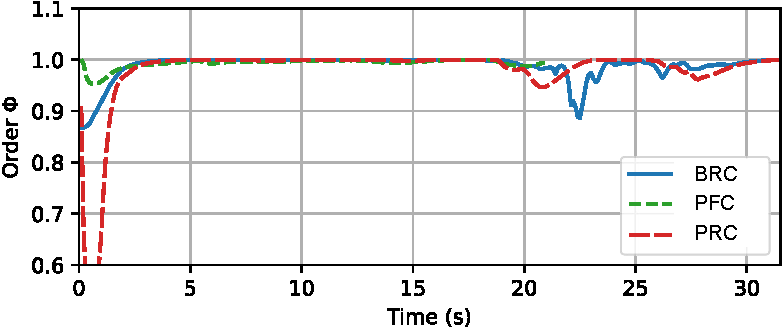
\includegraphics[width=\textwidth]{paper3/images/order_scen2.pdf}
    \caption{Scenario 2 - \textit{Order} $\Phi$}
    \label{fig:order2}
    \end{subfigure}
    \begin{subfigure}[b]{0.495\textwidth}
    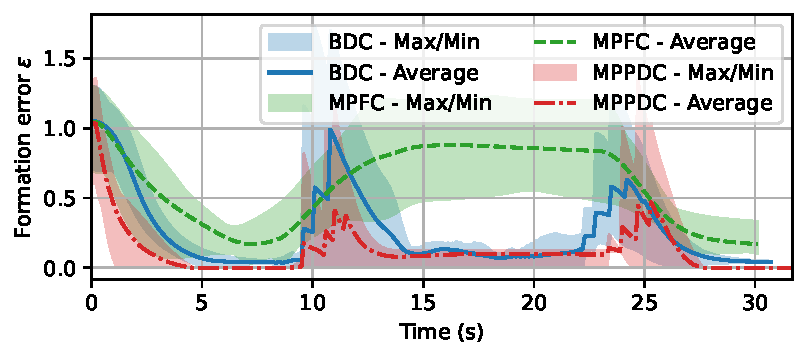
\includegraphics[width=\textwidth]{paper3/images/error_scen1.pdf}
    \caption{Scenario 1 - \textit{Formation error} $\varepsilon$}
    \label{fig:error1}
    \end{subfigure}
    \begin{subfigure}[b]{0.495\textwidth}
    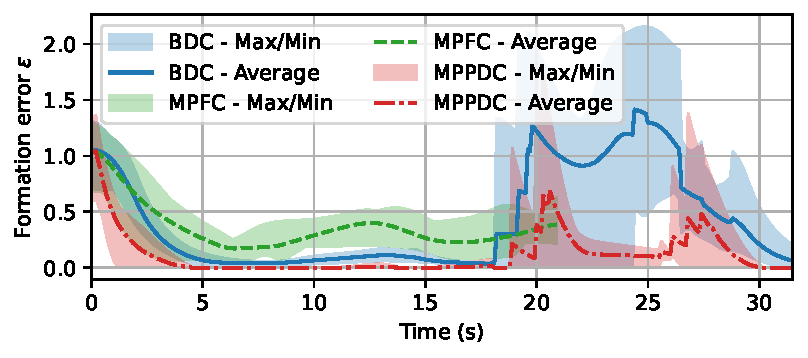
\includegraphics[width=\textwidth]{paper3/images/error_scen2.pdf}
    \caption{Scenario 2 - \textit{Formation error} $\varepsilon$}
    \label{fig:errorr2}
    \end{subfigure}
    \caption{Comparison results of three control methods in two scenarios.}
    \label{fig:comparison}
\end{figure*}

\begin{figure}
    \centering
    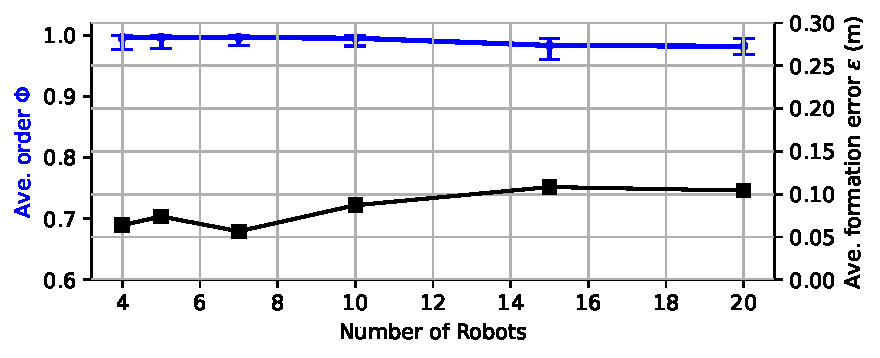
\includegraphics[width=0.8\textwidth]{paper3/images/scalability.pdf}
    \caption{Effect of the swarm size on system performance, including the mean \textit{order} $\Phi$ and formation error $\varepsilon$.}
    \label{fig:scalability}
\end{figure}

Figure \ref{fig:path} shows the formation results for both scenarios. After takeoff, the robots rapidly form the desired pentagon shape, then change their formation to pass through tight passages and finally transform back to the original desired shape. Figures~\ref{fig:cor1}-\ref{fig:cor2} depict the scaling factor $\kappa$ and the number of robots within each control mode during operation. When the environment's width is large, the scaling factor $\kappa$ stays at 1 to maintain the desired shape. As the environment narrows, $\kappa$ gradually decreases leading to more robots switching to \textit{``tailgating''} mode. The formation thus shrinks until $\kappa$ reaches 0, the point at which all robots are in \textit{``tailgating''} mode. Upon exiting the narrow corridor, $\kappa$ increases, allowing the formation to expand back to its original shape. The PRC hence provides reconfiguration capabilities for the robot swarm to adapt to complex environmental conditions.

\begin{table*}
\centering
\caption{Comparison between BRC, PFC, and the proposed PRC}
\label{tbl:analys}
\begin{tabular}{C{0.8cm}C{1.2cm}C{1.8cm}C{1.8cm}C{2.8cm}C{2.2cm}C{2.5cm}}
\hline \hline
Scen.             & Method & Success rate  & Mean \textit{order} $\Phi$ & Mean speed (m/s) ($v_\text{ref}=1$~m/s) & Mean formation error $\varepsilon$ (m) & Acceleration cost $\Gamma$ (m$^2$/s$^4$) \\ \hline
\multirow{3}{*}{1  } & BRC      & \textbf{10/10} & 0.9890     & 1.0249     & 0.3048               & 69.6589    \\
                     & PFC     & 8/10  & \textbf{0.9934}     & 1.0639     & 0.6376               & \textbf{23.7442}    \\
                     & PRC    & \textbf{10/10} & 0.9824     & \textbf{0.9863}     & \textbf{0.2423}               & 25.0894    \\ \hline
\multirow{3}{*}{2}   & BRC      & 6/10  & 0.9883     & \textbf{0.9887}     & 0.6872               & 53.8718    \\
                     & PFC     & 0/10  & \textbf{0.9953}     & 1.0470      & 0.4593               & \textbf{19.0365}    \\
                     & PRC    & \textbf{9/10}  & 0.9830     & 0.9800       & \textbf{0.3217}               & 21.8559   \\ \hline \hline
\end{tabular}
\end{table*}
 
Figure~\ref{fig:comparison} presents comparison results between the PRC and other control methods. In terms of speed, the proposed controller achieves more stable velocities with values closer to the reference $v_\text{ref}$ in both scenarios, as indicated via the average and maximum/minimum values shown in Figures~\ref{fig:speed1}-\ref{fig:speed2}. 
For the \textit{order} metric, the PRC exhibits large fluctuation at start but quickly converges to a high consensus among the robots with the \textit{order} value reaching 1, as shown in Figures~\ref{fig:order1}-\ref{fig:order2}. Both the BRC and PFC also perform well, although the BRC shows more variation than the PRC during the transition phase. In terms of formation maintenance, the PRC outperforms other methods with the smallest average error, as shown in Figures~\ref{fig:error1}-\ref{fig:errorr2}. These results are further confirmed in Table~\ref{tbl:analys}, which presents comparison data. The proposed PRC shows high performance in all metrics, with the highest success rate and the smallest formation error in both scenarios. The PFC fails in scenario 2 due to its limitation in reconfiguring the formation. The BRC has good performance in speed and mean order. It however introduces high acceleration costs, indicating that the method is not energy efficient.       

In another experiment, we vary the swarm size between 4, 5, 7, 10, 15, and 20 robots and measure the mean \textit{order} $\Phi$ and formation error $\varepsilon$ to evaluate the scalability of the proposed method. The result in Figure \ref{fig:scalability} shows that as the number of robots increases, the PRC maintains strong consensus among robots with a mean \textit{order} close to~1. The formation error, excluding the formation generation and the transition stage, remains low with variations around 0.05~m. The PRC is therefore scalable with stable performance across different swarm sizes.

\subsection{Software-in-the-loop verification}
\begin{figure*}
    \centering
    \begin{subfigure}[b]{0.56\textwidth}
    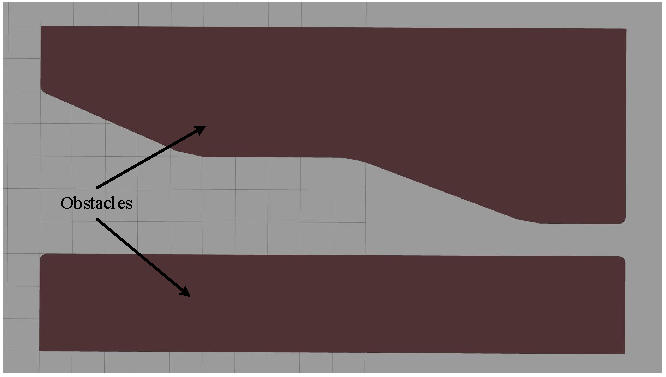
\includegraphics[width=\textwidth]{paper3/images/tunnel.pdf}
    \caption{The cave-like environment}
    \label{fig:gazebo_tunnel}
    \end{subfigure}
    \begin{subfigure}[b]{0.42\textwidth}
    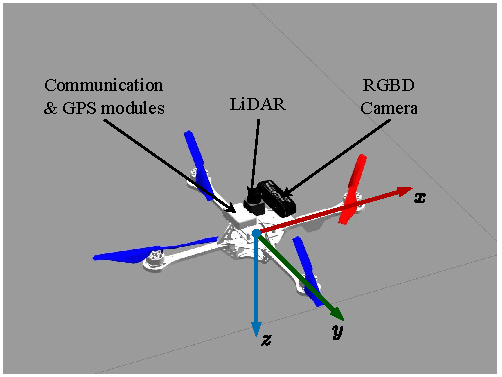
\includegraphics[width=\textwidth]{paper3/images/hummingbird.pdf}
    \caption{The drone model~\cite{Bui2022,Furrer2016}}
    \label{fig:gazebo_hummingbird}
    \end{subfigure}
    \caption{The robot and environment structure used for software-in-the-loop tests.}
    \label{fig:sil}
\end{figure*}
\begin{figure*}
    \centering
    \begin{subfigure}[b]{0.325\textwidth}
    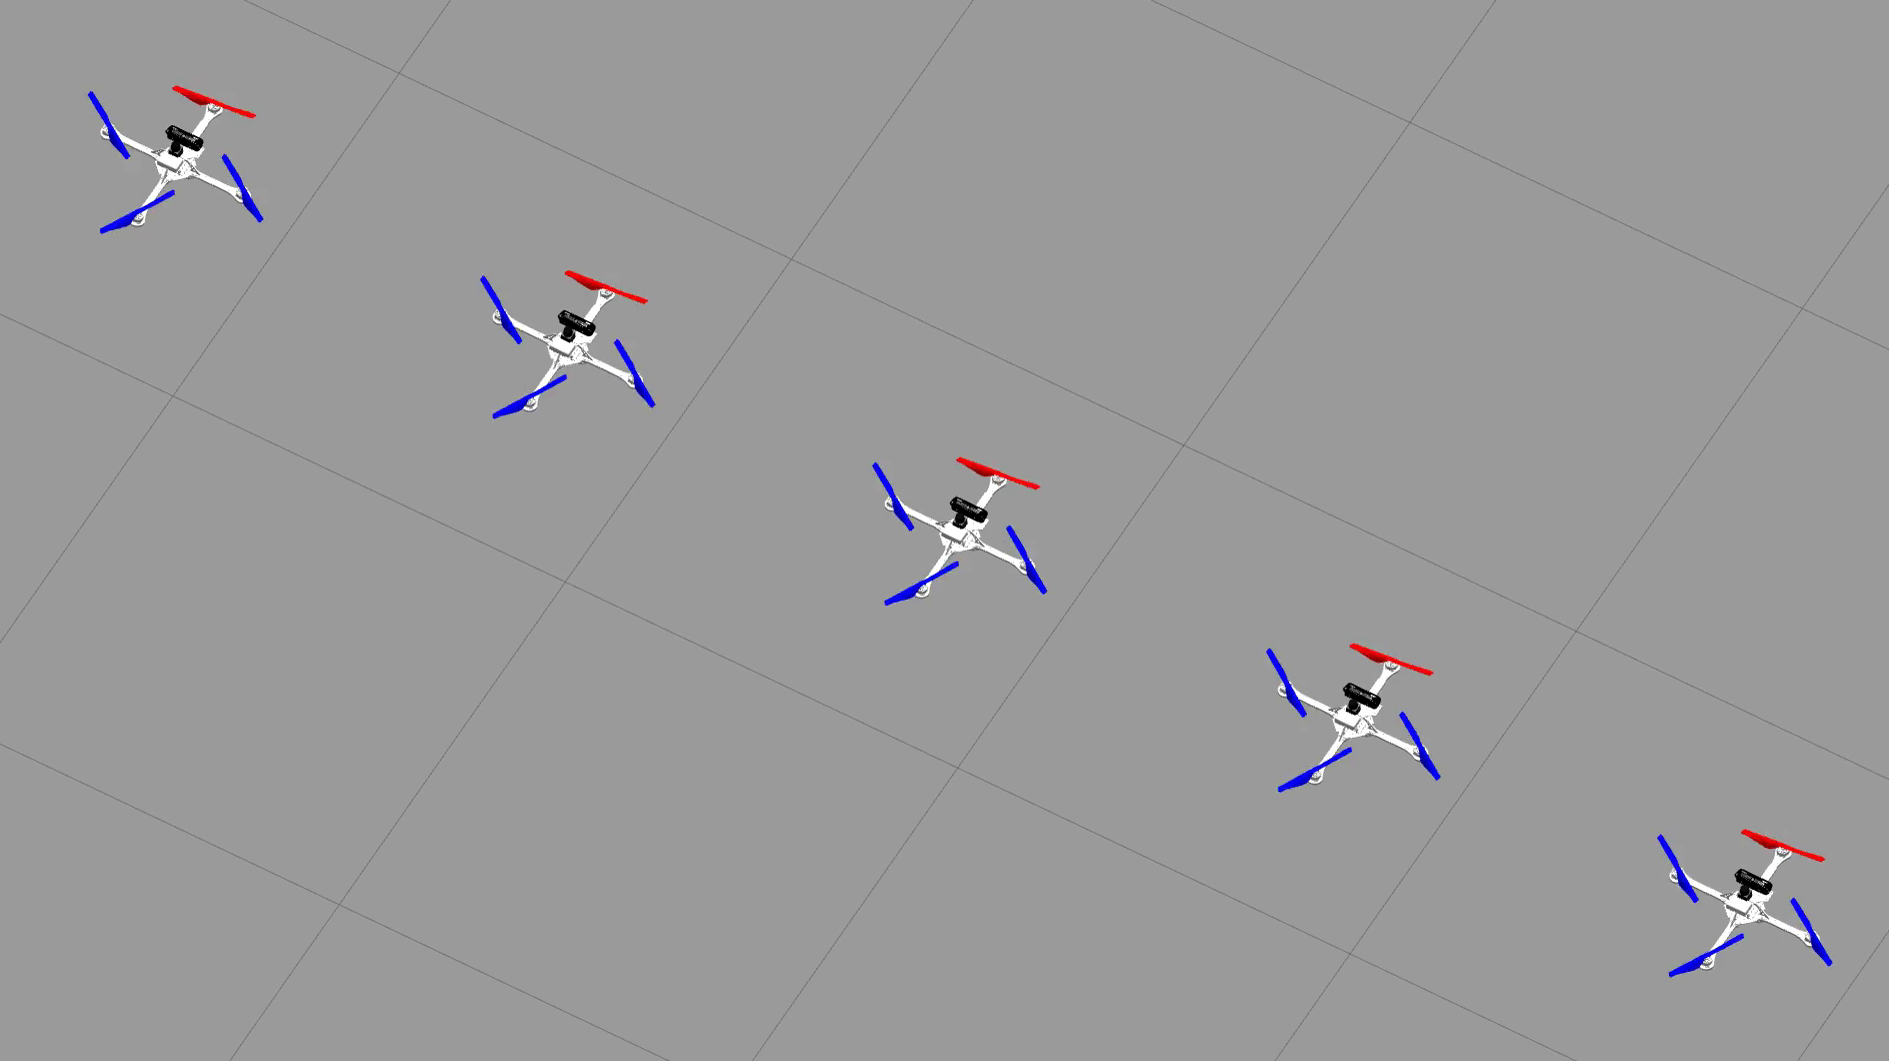
\includegraphics[width=\textwidth]{paper3/images/gazebo_01.png}
    \caption{}
    \end{subfigure}
    \begin{subfigure}[b]{0.325\textwidth}
    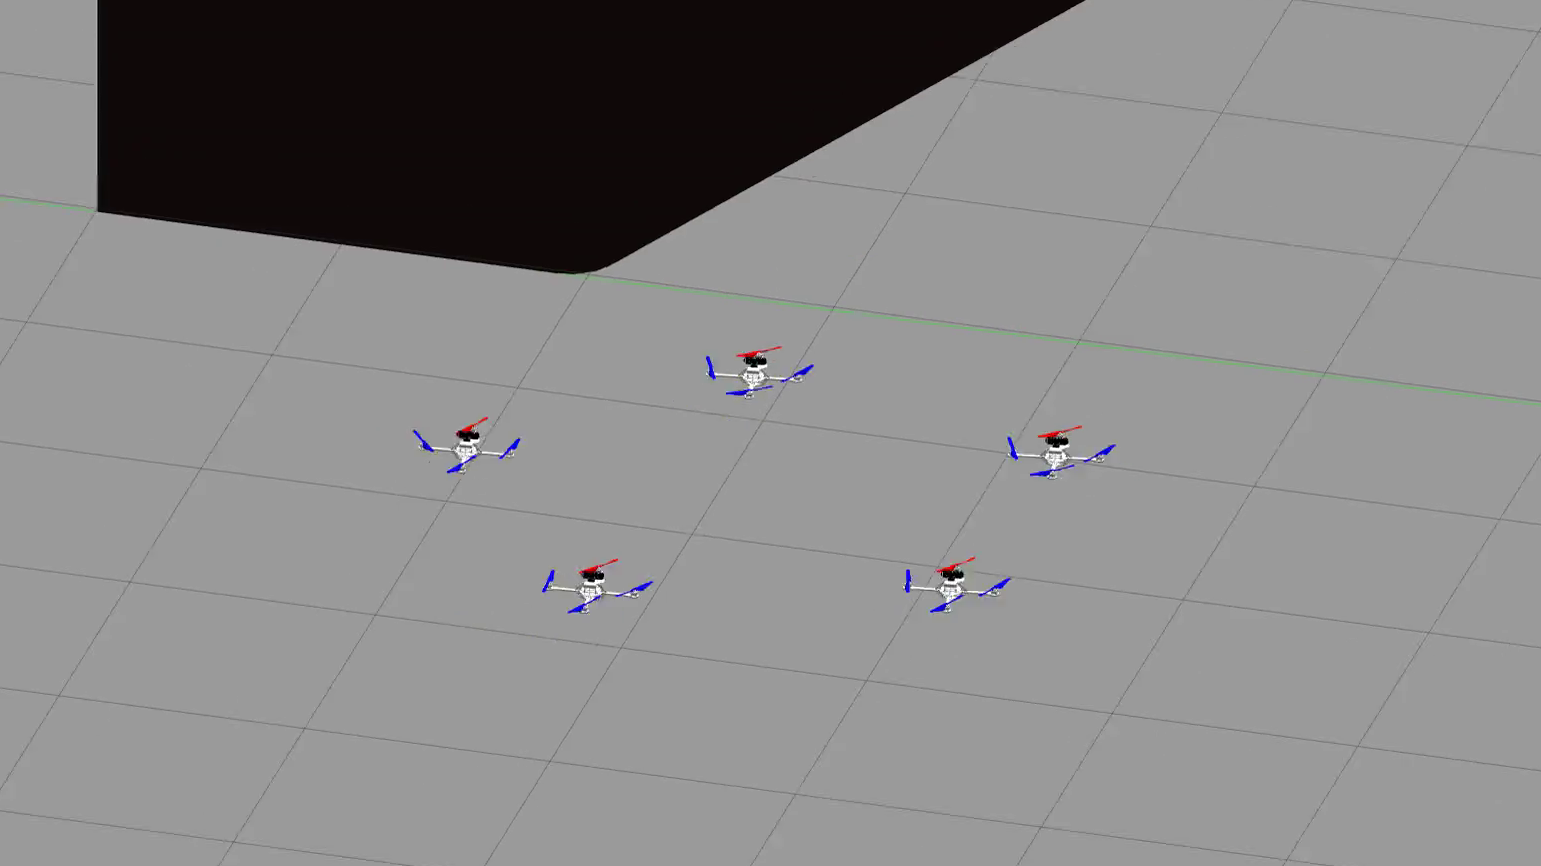
\includegraphics[width=\textwidth]{paper3/images/gazebo_02.png}
    \caption{}
    \end{subfigure}
    \begin{subfigure}[b]{0.325\textwidth}
    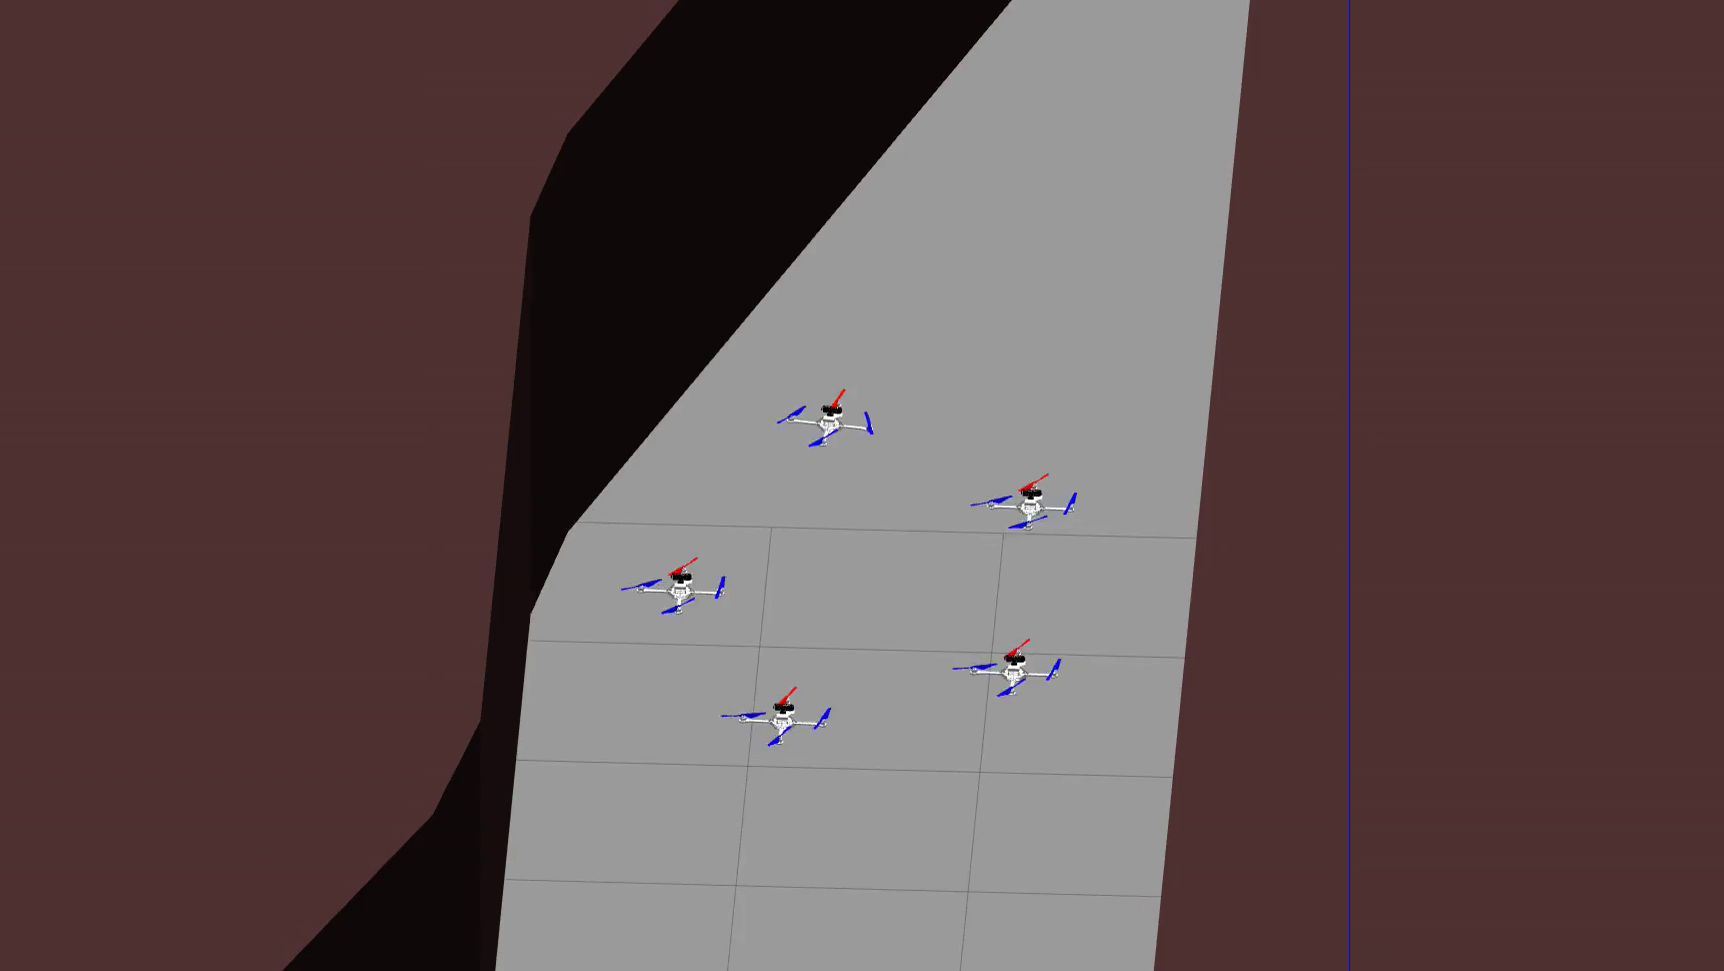
\includegraphics[width=\textwidth]{paper3/images/gazebo_03.png}
    \caption{}
    \end{subfigure}
    \begin{subfigure}[b]{0.325\textwidth}
    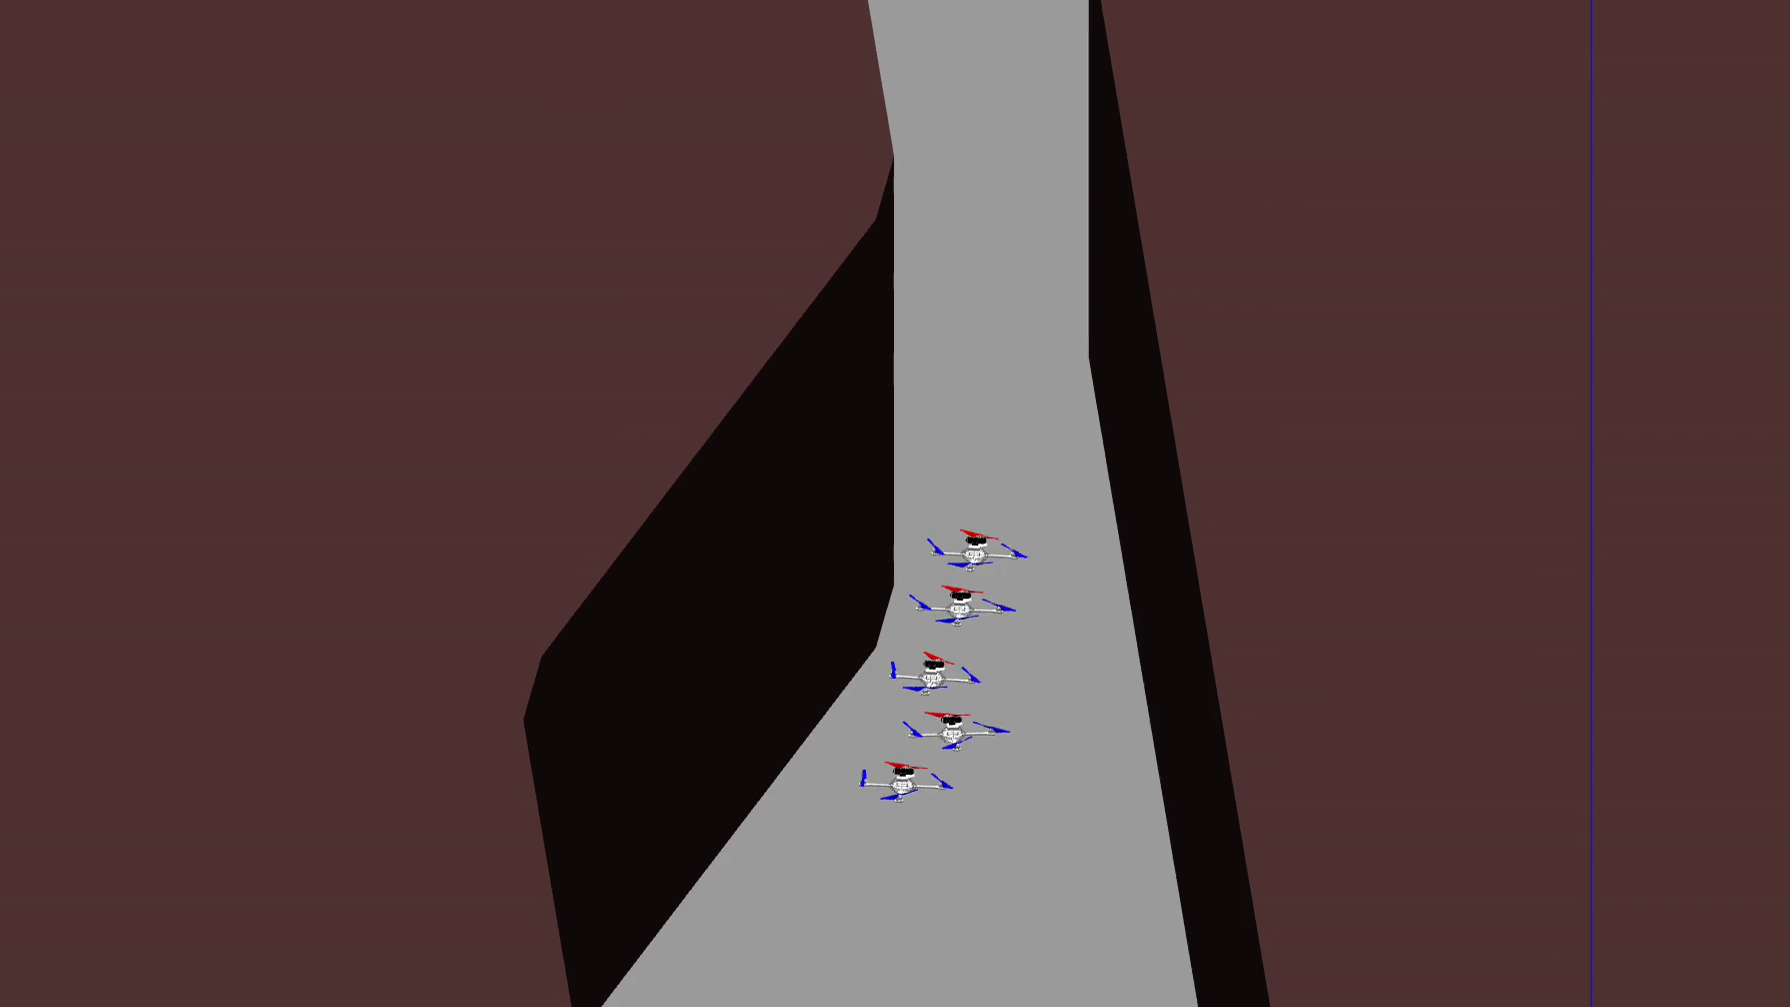
\includegraphics[width=\textwidth]{paper3/images/gazebo_04.png}
    \caption{}
    \end{subfigure}
    \begin{subfigure}[b]{0.325\textwidth}
    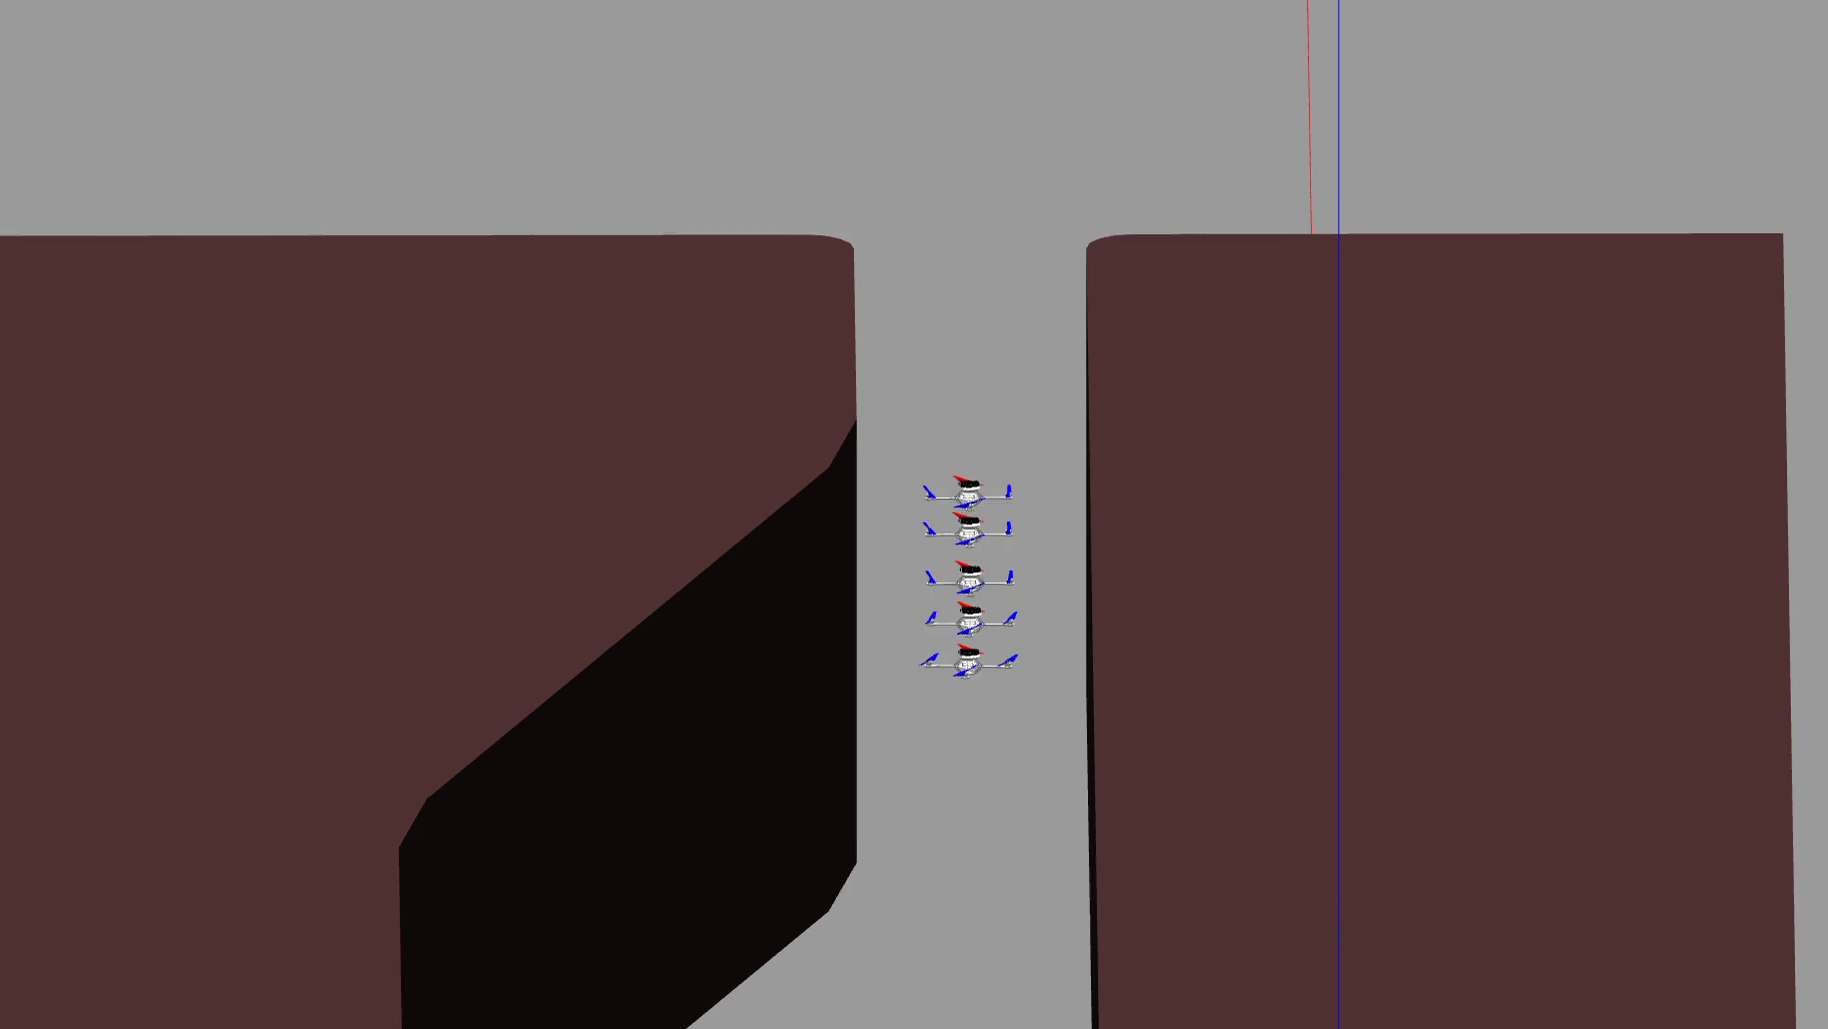
\includegraphics[width=\textwidth]{paper3/images/gazebo_05.png}
    \caption{}
    \end{subfigure}
    \begin{subfigure}[b]{0.325\textwidth}
    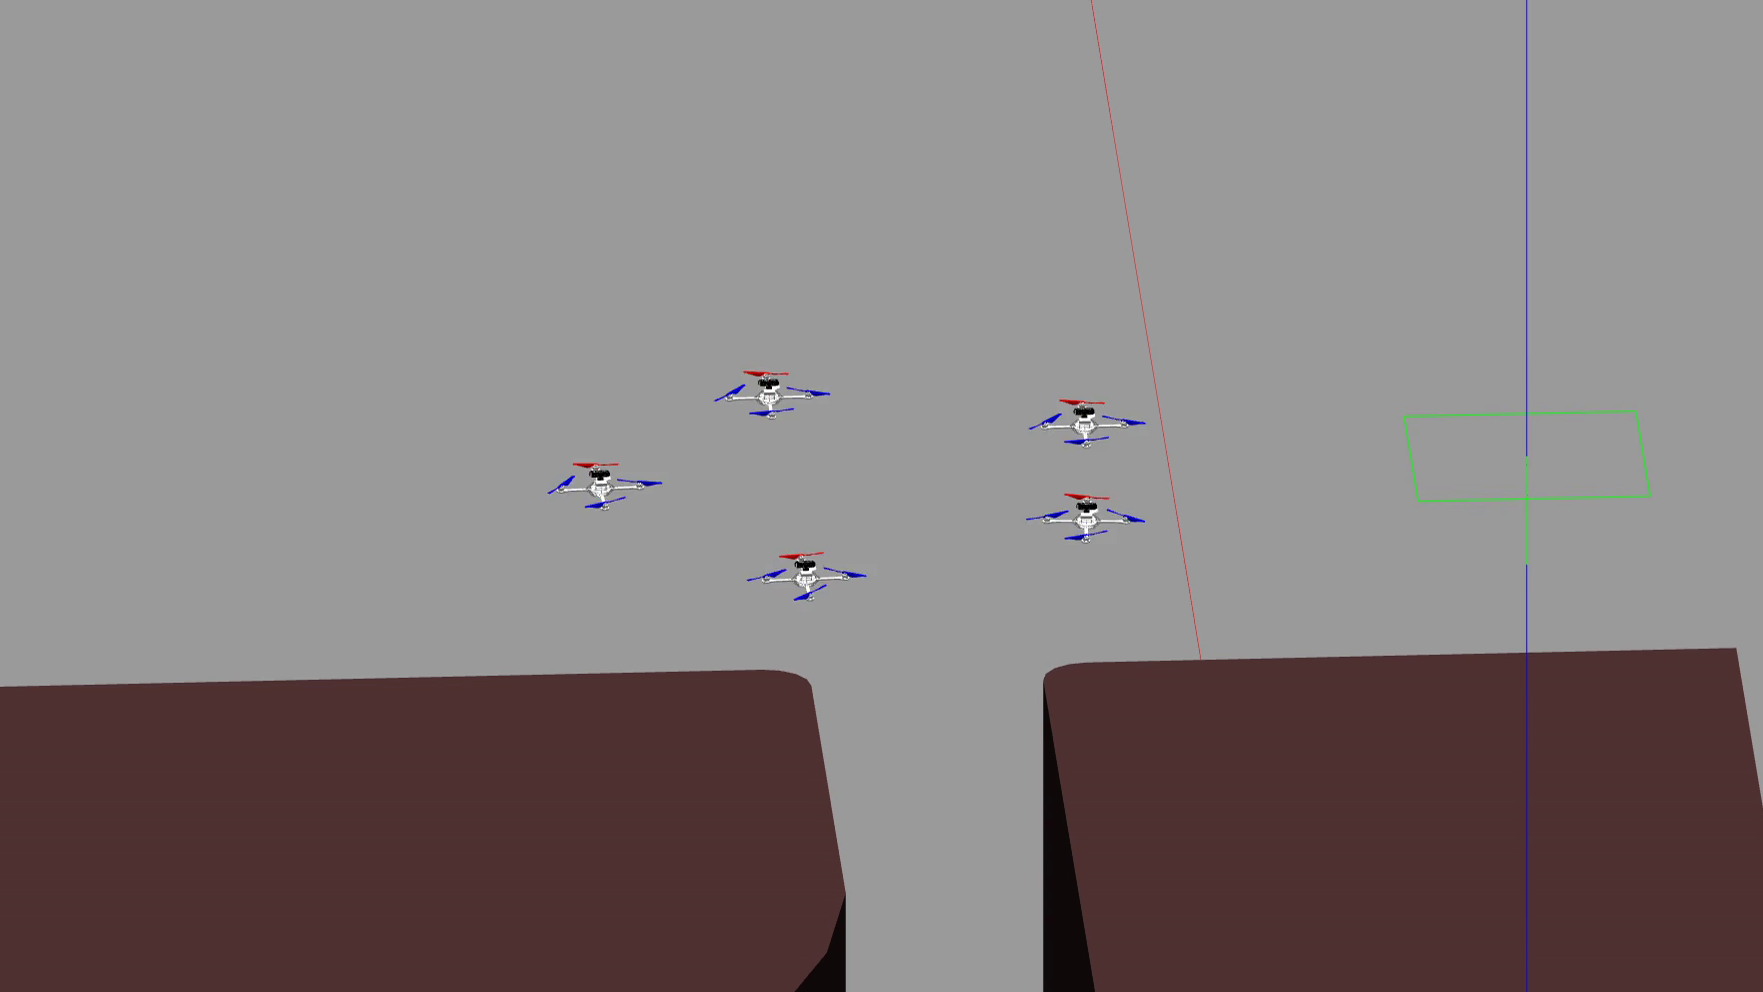
\includegraphics[width=\textwidth]{paper3/images/gazebo_06.png}
    \caption{}
    \end{subfigure}
    \caption{Reconfiguration process of the robot swarm in a SIL test: (a) initial positions of the robots; (b) form the desired pentagon shape; (c) shrink the formation in adaption to the environment; (d)-(e) switch to \textit{``tailgating''} mode to travel through the narrow passage; (f) transform back to the desired shape.}
    \label{fig:snap}
\end{figure*}

\begin{figure*}
    \centering
    \begin{subfigure}[b]{0.495\textwidth}
    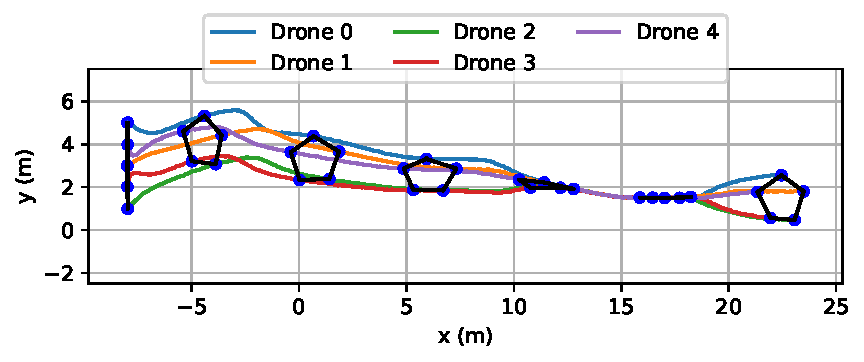
\includegraphics[width=\textwidth]{paper3/images/gazebo_path.pdf}
    \caption{The formation and motion paths}
    \label{fig:gazebo_path}
    \end{subfigure}
    \begin{subfigure}[b]{0.495\textwidth}
    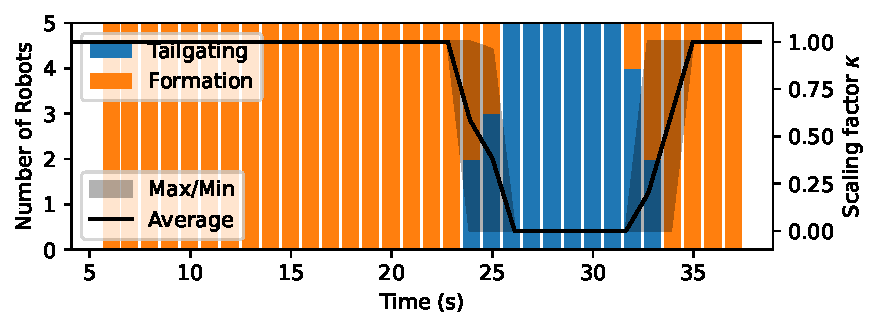
\includegraphics[width=\textwidth]{paper3/images/gazebo_correlation.pdf}
    \caption{Number of robots and scaling factor $\kappa$}
    \label{fig:gazebo_mode}
    \end{subfigure}
    \begin{subfigure}[b]{0.495\textwidth}
    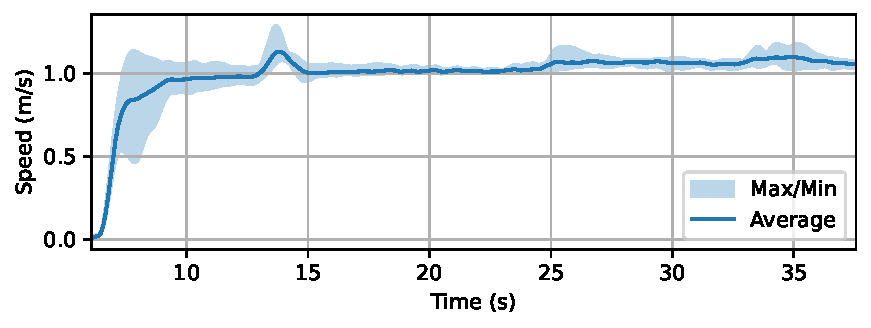
\includegraphics[width=\textwidth]{paper3/images/gazebo_speed.pdf}
    \caption{The speed profile}
    \label{fig:gazebo_speed}
    \end{subfigure}
    \begin{subfigure}[b]{0.495\textwidth}
    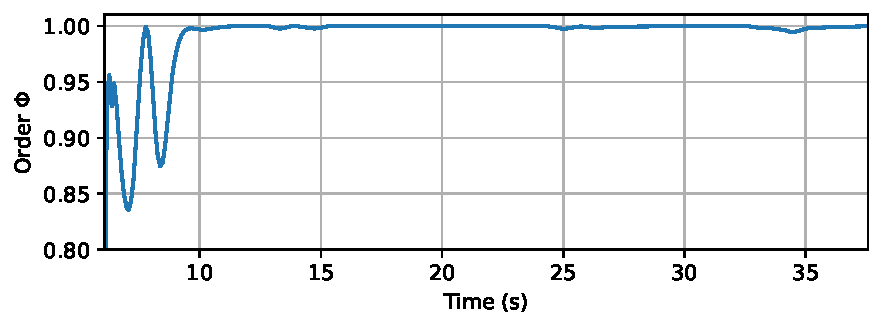
\includegraphics[width=\textwidth]{paper3/images/gazebo_order.pdf}
    \caption{The \textit{order} metric $\Phi$}
    \label{fig:gazebo_order}
    \end{subfigure}
    \begin{subfigure}[b]{0.495\textwidth}
    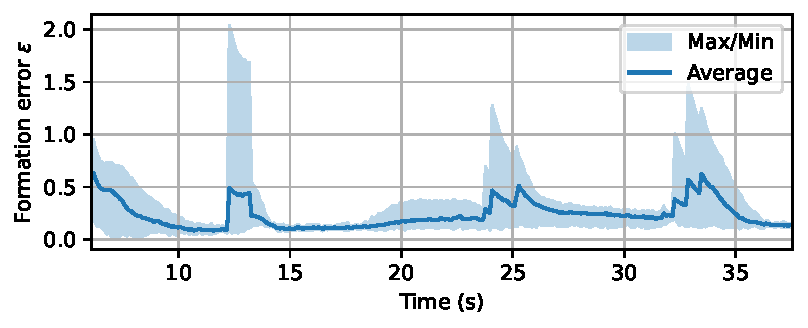
\includegraphics[width=\textwidth]{paper3/images/gazebo_error.pdf}
    \caption{The \textit{formation error} $\varepsilon_i$}
    \label{fig:gazebo_error}
    \end{subfigure}
    \begin{subfigure}[b]{0.495\textwidth}
    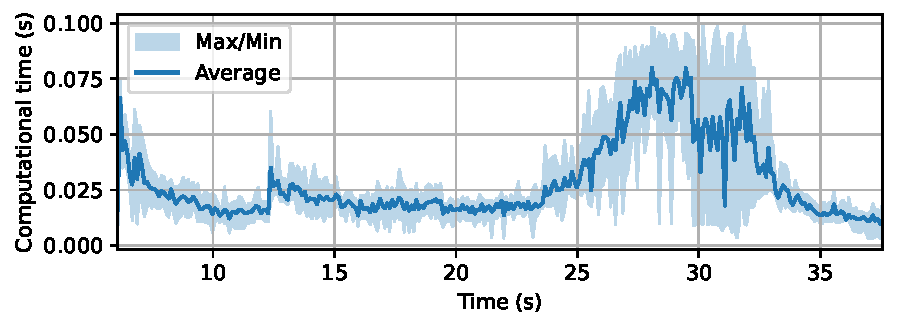
\includegraphics[width=\textwidth]{paper3/images/gazebo_computation.pdf}
    \caption{The computational time}
    \label{fig:gazebo_time}
    \end{subfigure}
    \caption{Results of the SIL tests}
    \label{fig:gazebo}
\end{figure*}

We have carried out software-in-the-loop (SIL) tests to evaluate the performance of the proposed controller in practical conditions. The environment is a narrow space that consists of two large obstacles forming a cave-like structure as shown in Figure~\ref{fig:gazebo_tunnel}. The robots include five homogeneous Hummingbird quadrotors\footnote{Source code used to setup SIL tests in Gazebo - {\tt\url{https://github.com/duynamrcv/hummingbird_simulator}}} obtained from the RotorS simulator~\cite{Furrer2016} with an arm length of 0.17~m, a mass of 0.716~kg, the rotor thrust constant of $1.6\time10^{-2}$~N/A, and the rotor drag constant of $8.54858\times10^{-6}$~Nm/A, as depicted in Figure~\ref{fig:gazebo_hummingbird}. Each robot is equipped with a range sensor to collect point cloud data of the environment, a positioning module for localization, and a communication module to interact with other robots.

Figure~\ref{fig:snap} presents the formation reconfiguration process as the swarm navigates through the environment. The robots continuously collect data about the environment and based on it adjust their formation to ensure safe operation. Figure~\ref{fig:gazebo} provides a detailed view of the result. Each UAV determines its mode and desired position based on the perception of the surrounding environment and information about its neighbors. The robots together form the relevant shape in a decentralized manner, as shown in Figures~\ref{fig:gazebo_path} - \ref{fig:gazebo_mode}. Requirements for speed, order, and formation accuracy are also met, as depicted in Figures~\ref{fig:gazebo_speed} - \ref{fig:gazebo_error}. Moreover, the computational time per controller iteration, shown in Figure~\ref{fig:gazebo_time}, indicates that the system can operate at a sampling rate of 10 Hz in the worst-case scenario, which is sufficient for real-time robot operation.

\subsection{Discussion}
Evaluation and comparison results show the key properties of the proposed control method as follows:

\subsubsection{Decentralization} The PRC is fully decentralized as each robot makes decisions based solely on its own sensor data and information from its neighbors. Unlike the approach in~\cite{AlonsoMora2018}, which requires system-wide communication to obtain information on all robots, the PRC utilizes only one-hop communication between the robot and its neighbors to update predictive states.

\subsubsection{Reliability}

The PRC can navigate the robots through complex environments with desirable performance metrics such as low formation error, stable formation direction, and high speed. Unlike previous studies ~\cite{Elkilany2020,Vsrhelyi2018,Soria2021,AlonsoMora2018} which only shrink or expand the formation to adapt to environment variations, the PRC enables the robots to completely transform to a new formation to safely maneuver through tight spaces.

\subsubsection{Scalability}
The PRC can operate with different swarm sizes, for example from 4 to 20 robots, without requiring any modifications to the algorithm. It maintains reliable performance and consistent metric values across various swarm sizes. 

\subsubsection{Robustness}
The PRC provides robustness to operate in different environmental structures. Through real-time data obtained from local sensors and communication networks, the swarm can dynamically expand, shrink, or transform into a line shape to optimize its ability to navigate through narrow spaces.